\scanpage{37}
\margin{36}
le carré est
\[
 \lambda=\frac{(\xi+\eta)^2}{\xi\wedge\eta}
 =\deleted{\unsure{\frac{\xi}{\eta}}}\frac{\xi}{\eta}+\frac{\eta}{\xi}+2
\]
et dont la connaissance nous permet de retrouver la situation de départ à iso.
\uline{\unsure{un|aux}} \uline{unique} près. La condition à mettre sur
$\lambda$ est que $\lambda-4\ne0$ i.e.
\[
 \lambda'\overset{\unsure{\mathrm{df}}}{=}\lambda-
 2= \frac{\xi}{\eta}+\frac{\eta}{\xi}\ne2
\]
En termes d'une base \deleted{\unsure{de}} $e_1$ de $L_1$,
satisfaisant $e_1^4=e=\xi\wedge\eta$, donnant une base $e_1^2$ de $L_2$,
la situation est déterminée par \inserted{la paire d'éléments distincts}
$\xi_0,\eta_0\in\mathbb C$ $(\xi=\xi_0e_1^2,\ \eta=\eta_0e_1^2)$,
satisfaisant $\xi_0\eta_0=1$, ou encore par
$\mu=\xi_0+\eta_0\inserted{\in\mathbb C}$, satisfaisant $\mu^2-4\ne0$,
$\xi_0$ et $\eta_0$ se récupérant comme solutions de l'équation
\[
 z^2-\mu z+1=0,
\]
l'équation \tikz[baseline=(ineq.base)]{
\node[inner sep=1pt] (ineq) {$\mu^2-4\ne0\quad\text{i.e.}\quad\unsure{\mu^2|\mu}\ne\pm2$};
\draw ([xshift=-2pt,yshift=4pt]ineq.south west)
 .. controls ([xshift=-2pt,yshift=-2pt]ineq.south west) and
 ([xshift=-1pt,yshift=-3pt]ineq.south west) .. ([xshift=2pt,yshift=-3pt]ineq.south west)
 -- ([xshift=-2pt,yshift=-3pt]ineq.south east)
 .. controls ([xshift=1pt,yshift=-3pt]ineq.south east) and
 ([xshift=2pt,yshift=-1pt]ineq.south east) .. ([xshift=2pt,yshift=1pt]ineq.south east);
\draw ([xshift=5pt,yshift=2pt]ineq.south east) -- ([xshift=5pt,yshift=2pt]ineq.north east);
}
s'exprime par les \inserted{2} solutions sont distinctes (néc\textsuperscript{t} non nulles car leur
produit est $1$). \deleted{\unsure{Les}} On récupère $I$ comme l'ens des solutions de
\[
 z^4-\mu z^2+1=0
\]
\[
 I=\left\{\pm\sqrt{\tfrac12\left(\mu\pm\sqrt{\mu^2-4}\right.}\right\}
 =\left\{\pm\sqrt{\mu'\pm\sqrt{\mu'^2-1}}\right\}
\]
\margin{\begin{tikzpicture}[baseline=(eq.base)]
\node[inner sep=1pt] (eq) {où $\mu'=\tfrac12\mu$};
\node[anchor=west,inner sep=1pt] (ie) at (eq.east) {i.e.};
\draw ([xshift=-2pt]eq.west)
 .. controls ([xshift=2pt,yshift=3pt]eq.north west) and
 ([xshift=-4pt,yshift=4pt]eq.north east) .. ([xshift=0pt,yshift=2pt]eq.north east)
 .. controls ([xshift=2pt]eq.north east) and
 ([xshift=-2pt,yshift=-2pt]ie.south west) .. ([xshift=2pt,yshift=-2pt]ie.south west)
 -- ([yshift=-2pt]ie.south east);
\end{tikzpicture}}
